\documentclass{beamer}
\definecolor{links}{HTML}{2A1B81}

\usepackage[utf8]{inputenc}
\usepackage[norsk]{babel}
\usepackage{hyperref}
\hypersetup{
  colorlinks=true,
  linkcolor=,
  urlcolor=links
}

\usetheme{Copenhagen}
\usecolortheme{seahorse}

\definecolor{DMMH}{HTML}{F9F5EB}

\setbeamercolor{palette primary}{bg=DMMH,fg=black}
\setbeamercolor{palette secondary}{bg=DMMH,fg=black}
\setbeamercolor{palette tertiary}{bg=DMMH,fg=black}
\setbeamercolor{palette quaternary}{bg=DMMH,fg=black}

\title{Litteratursøkekurs}
\author{Thomas Rambø\inst{1}}
\institute[DMMH-biblioteket]{
  \inst{1}
  Biblioteket\\
  Dronning Mauds Minne Høgskole
}

\date[DMMH 2018]{DMMH, høsten 2018}
\logo{
\includegraphics[height=1cm]{../media/logo.png}}

\AtBeginSection[]
{
  \begin{frame}
    \frametitle{Innhold}
    \tableofcontents[currentsection]
  \end{frame}
}

\begin{document}

\frame{\titlepage}
\begin{frame}
  \frametitle{Innhold}
  \tableofcontents
\end{frame}

\section{Bakgrunnskunnskap}
\subsection{Felt}
\begin{frame}
  \frametitle{Felt}
  \begin{columns}
    \column{0.5\textwidth}
    \begin{itemize}
    \item \href{https://en.wikipedia.org/wiki/Field_(computer_science)}{Felt} er informasjonsbitene som er knyttet til bestemte materialer.
    \item \alert{Forfatter}, \alert{tittel}, \alert{utgivelsesår} er eksempler på felt.
    \end{itemize}

    \column{0.5\textwidth}
    \centering
    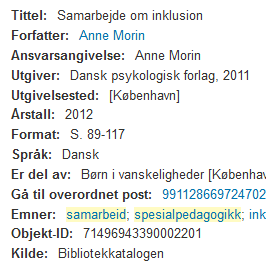
\includegraphics[width=0.8\textwidth]{../media/felt-i-oria.png}
  \end{columns}
\end{frame}

\subsection{Kontrollerte emneord}
\begin{frame}
  \frametitle{Kontrollerte emneord}
  \begin{columns}
    \column{0.5\textwidth}
    \centering
    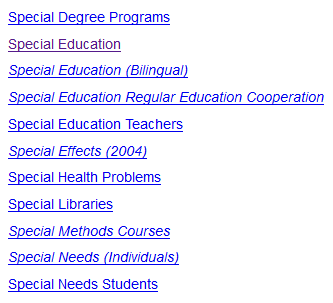
\includegraphics[width=0.8\textwidth]{../media/kontrollerte-emneord.png}

    \column{0.5\textwidth}
    \begin{itemize}
    \item \href{https://snl.no/emneord}{Kontrollerte emneord} er bestemte navneformer på bestemte emner.
    \item Også kalt tesaurustermer eller deskriptorer.
    \end{itemize}
  \end{columns}
\end{frame}

\section{Søk med kontrollerte emneord}
\begin{frame}
  \frametitle{Søk med kontrollerte emneord}
  \begin{itemize}
  \item \alert{Feltet} for emne bruker i flere litteraturdatabaser \alert{kontrollerte emneord}, og man kan utnytte dette til å finne litteratur om et bestemt emne.
  \item Siden emneordene er kontrollerte kan man finne de fleste relevante artikler.
  \end{itemize}
\end{frame}
\subsection{Kontrollerte emneord i ERIC}
\begin{frame}
  \frametitle{Kontrollerte emneord i ERIC}
  \begin{quote}
    The ERIC Thesaurus is a list of terms representing research topics in the field of education. Descriptors from the ERIC Thesaurus are \alert{assigned to every document} in the ERIC digital library to describe its subject content.
  \end{quote}
\end{frame}
\begin{frame}
  \centering
  
\includegraphics[width=1\textwidth]{../media/eric-descriptor.png}
\end{frame}
\begin{frame}
  \centering
  
\includegraphics[width=1\textwidth]{../media/eric-descriptor-2.png}
\end{frame}

\section{Søk med nøkkelord og fulltekstsøk}
\begin{frame}
  \frametitle{Søk med nøkkelord og fulltekstsøk}
  \begin{itemize}
  \item Søk med nøkkelord og fulltekstsøk blir gjort i \alert{alle felt} (tittel, forfatter, emne) og i \alert{innholdet} til artikkelen.
  \item Aktuelle søketjenester er \href{http://bibsys-almaprimo.hosted.exlibrisgroup.com/primo_library/libweb/action/search.do?vid=DMMH}{Oria}, \href{https://scholar.google.com}{Google Scholar} og \href{http://apps.webofknowledge.com}{Web of Science}.
  \end{itemize}
\end{frame}

\begin{frame}
  \frametitle{Når burde man velge nøkkelord og fulltekstsøk?}
  Nøkkelord- og fulltekstsøk er gunstige når man ønsker å inkludere mest mulig materiale blant søkeresultatene.
\end{frame}

\subsection{Nøkkelordsøk i Google Scholar}
\begin{frame}
  \frametitle{Nøkkelordsøk i Google Scholar}
  \begin{itemize}
  \item Med Google Scholar kan du søke på tittel, forfatter, år, utgiver, tekstinnhold, osv.
  \item Søker i norske og internasjonale kilder, i alle sjangre.
  \end{itemize}
\end{frame}

\begin{frame}
  \begin{itemize}
  \item Nøkkelordsøk er standardsøket i Google Scholar.
  \item Begynn å taste nøkkelord adskilt med mellomrom for å få forslag til søk.
  \end{itemize}

  \centering
  
\includegraphics[width=0.8\textwidth]{../media/google-scholar.png}
\end{frame}

\end{document}
